\subsubsection{Sprint goal}
Per lo sprint è stata pianificata l'implementazione delle epiche riguardanti i giochi televisivi (\textit{L'Eredità} e \textit{Reazione a Catena}) e
l'inizio dell'epica riguardante gli scacchi.\\
In particolare sono state previste le seguenti funzionalità:
\begin{itemize}
    \item Visualizzare gli utenti che tentano di indovinare la parola del giorno
    \item Visualizzare la parola vincente
    \item Visualizzare gli utenti che indovinano la parola
    \item Visualizzare la posizione degli utenti che tentano di indovinare
    \item Possibilità di muovere le proprie pedine su una scacchiera
\end{itemize}


\subsubsection{Backlog}
\userstory%
{Come spettatore de \#leredita,\\voglio raccogliere i tweet di chi prova a indovinare la \textit{Ghigliottina},\\per visualizzare, in ordine temporale, tutti coloro che provano ad indovinare.}%
{5\\(2 frontend + 3 backend)}%
{Possibilità di visualizzare una pagina con tutti i tweet di tutte le persone che usano \#leredita e provano ad indovinare la \textit{Ghigliottina}.}%
{Cercando per data, verificare che vengano visualizzati i tentativi del giorno.}
{L'Eredità}

\userstory%
{Come spettatore de \#leredita,\\voglio visualizzare, su una mappa, la posizione di tutti coloro che provano ad indovinare\\per conoscere la posizione dei giocatori.}%
{4\\(4 frontend)}%
{Possibilità di visualizzare una pagina con tutte le posizioni su una mappa dei tweet di tutte le persone che usano \#leredita e provano ad indovinare la \textit{Ghigliottina}.}%
{Manualmente verificare che nella mappa siano presenti i marker dei tweet con la geolocalizzazione.}
{L'Eredità}

\userstory%
{Come spettatore de \#leredita,\\voglio visualizzare tutti coloro che indovinano la \textit{Ghigliottina}\\per sapere chi ha indovinato.}%
{7\\(4 frontend + 3 backend)}%
{Possibilità di visualizzare la parola del giorno assieme a tutti i vincitori che hanno indovinato.}%
{Cercando per data, verificare che venga trovata la parola del giorno.}
{L'Eredità}

\userstory%
{Come spettatore di \#reazioneacatena,\\voglio raccogliere i tweet di chi prova a indovinare l'ultima parola,\\per visualizzare, in ordine temporale, tutti coloro che provano ad indovinare.}%
{2\\(2 backend)}%
{Possibilità di visualizzare una pagina con tutti i tweet di tutte le persone che usano \#reazioneacatena e provano ad indovinare la parola finale.}%
{Cercando per data, verificare che vengano visualizzati i tentativi del giorno.}
{Reazione a catena}

\userstory%
{Come spettatore di \#reazioneacatena,\\voglio visualizzare, su una mappa, la posizione di tutti coloro che provano ad indovinare\\per conoscere la posizione di giocatori.}%
{0\\Segue dalla US de \#leredita}%
{Possibilità di visualizzare una pagina con tutte le posizioni su una mappa di tweet di tutte le persone che usano \#reazioneacatena e provano ad indovinare la parola finale.}%
{Manualmente verificare che nella mappa siano presenti i marker dei tweet con la geolocalizzazione.}
{Reazione a catena}

\userstory%
{Come spettatore de \#reazioneacatena,\\voglio visualizzare tutti coloro che indovinano l'ultima parola\\per sapere chi ha indovinato.}%
{2\\(2 backend)}%
{Possibilità di visualizzare la parola del giorno assieme a tutti i vincitori che hanno indovinato.}%
{Cercando per data, verificare che venga trovata la parola del giorno.}
{Reazione a catena}

\userstory%
{Come giocatore di scacchi,\\voglio poter muovere una pedina\\per fare la mia mossa.}%
{12\\(6 frontend + 6 backend)}%
{Possibilità di fare una mossa a scacchi e visualizzarla.}%
{Provare a effettuare mosse valide e invalide.}
{Scacchi}


\newpage
\subsubsection{Esito sprint}
Lo sprint è terminato con la conclusione di tutte le user stories pianificate.\\
\begin{figure}[H]
    \centering
    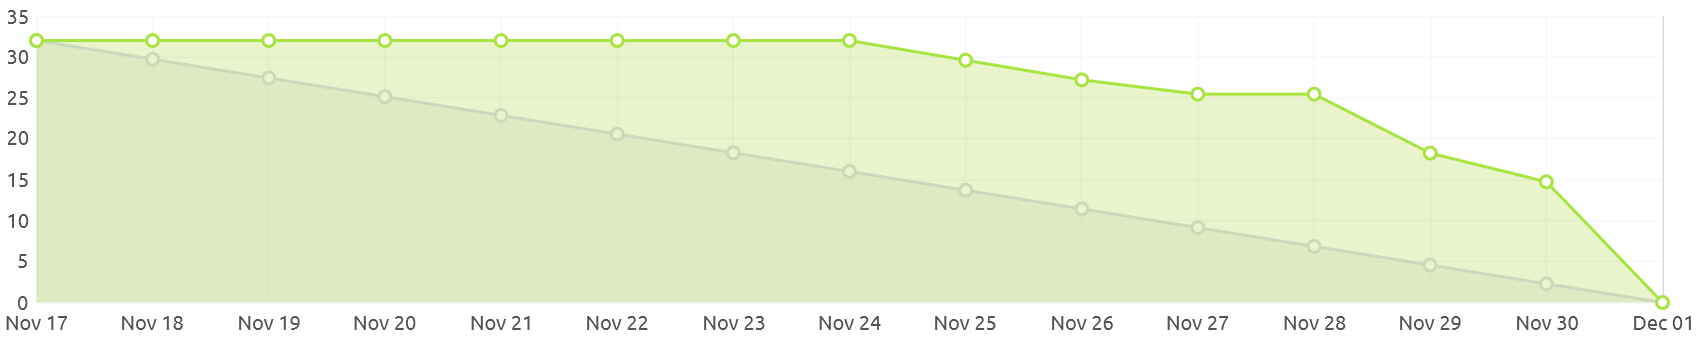
\includegraphics[width=15cm]{./img/sprint3/burndown.png}
    \caption{Burndown sprint 3}
\end{figure}
Il lavoro è stato però distribuito in maniera disomogenea, infatti, nella prima metà dello sprint non sono stati fatti progressi significativi,
mentre tutto il valore è stato portato nella seconda metà dello sprint. 
Conseguentemente anche le ore di lavoro sono tutte distribuite nel secondo periodo dello sprint.\\
Il monte ore obiettivo non è stato raggiunto, ma ciò era atteso in quanto durante lo sprint planning era già stata prevista una minore quantità di lavoro.
\begin{figure}[H]
    \centering
    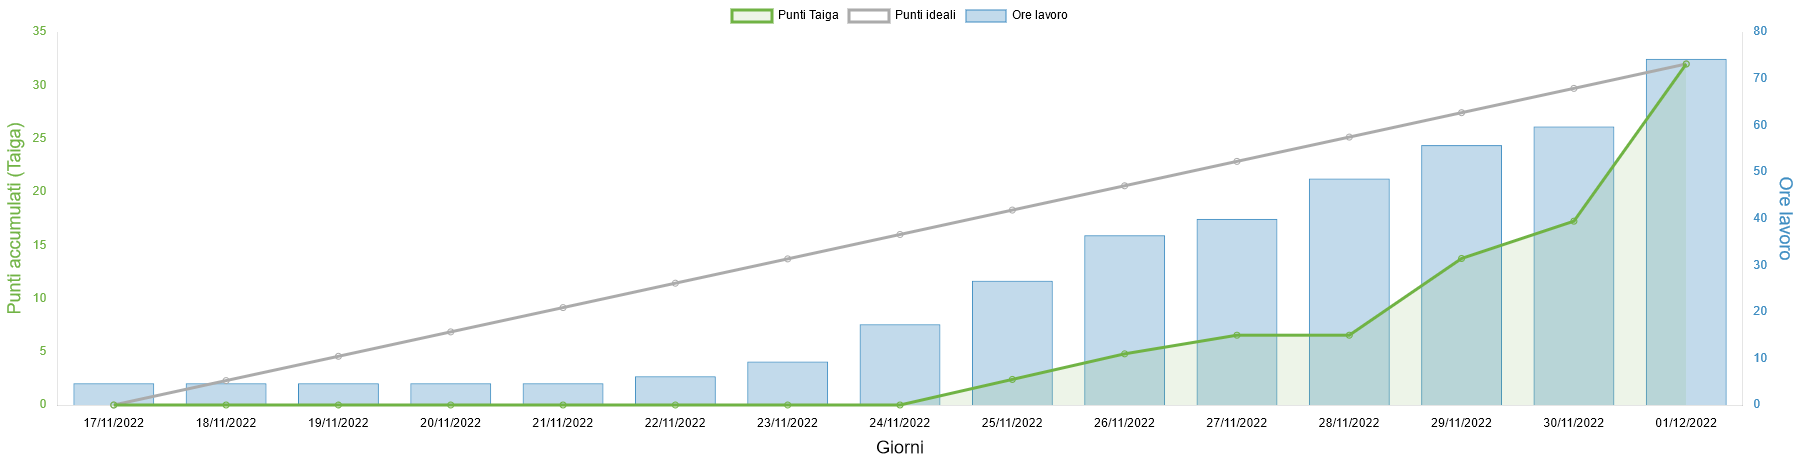
\includegraphics[width=15cm]{./img/sprint3/worktime.png}
    \caption{Progresso dei punti (asse a sinistra) e ore di lavoro (asse a destra)}
\end{figure}


\subsubsection{Sprint review}
Alla sprint review il cliente ha espresso le seguenti richieste:
\begin{itemize}
    \item Revisione del grafico a barre della frequenza dei tweet in situazioni in cui sono presenti solo tweet di una giornata
    \item Aggiungere ai giochi televisivi la visualizzazione dei giocatori più vincenti in un periodo di tempo
\end{itemize} 
Inoltre è stata aggiunta alle specifiche, con priorità massima, l'implementazione di funzionalità riguardanti il Fantacitorio.


\newpage
\subsubsection{Retrospettiva}
Dalla retrospettiva sono emerse le seguenti problematiche:
\begin{itemize}
    \item Abbiamo sottovalutato lo sprint e lavorato poco di conseguenza
    \item La DoD di alcune user stories risultavano ambigue
\end{itemize}
\begin{figure}[H]
    \centering
    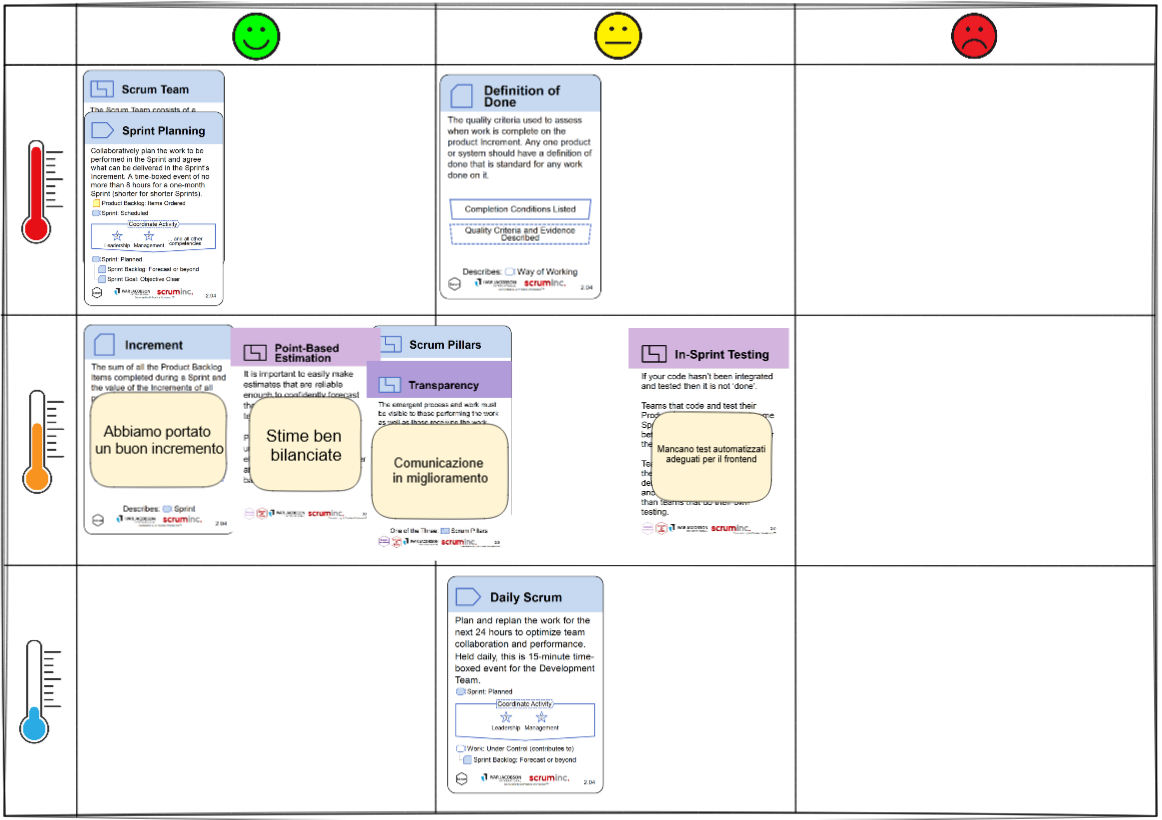
\includegraphics[width=15cm]{./img/sprint3/retrospettiva.png}
    \caption{Retrospettiva del 02/12/2022}
\end{figure}
